\begin{savequote}[6cm]
<< Don't you use your fancy mathematics to muddle the issue! >>
\qauthor{Applejack}
\end{savequote}

\chapter{Astral : Modèle théorique de requêtes continues}\label{chap:contrib:astral}
\chaptertoc

La gestion de flux de données est un domaine dérivé de la gestion de base de données relationnelles. Afin de définir un langage de requête uniforme pour pouvoir interroger autant les flux que les relations, il est nécessaire définir un modèle algébrique précis. Une grande importance est accordée au déterminisme du modèle. Dans certains cas, certaines formalisations ne définissent pas complètement les réponses aux requêtes. De ce fait, différentes évaluations d'une même requête peuvent retourner des ensembles de résultats différents. Nous souhaitons formaliser exactement les bases de l'algèbre afin de pouvoir fédérer les modèles existants.

Nous développons dans ce chapitre les fondations de notre algèbre : \textit{Astral} (\textit{Advanced Stream Algebra}). Cette algèbre reprend des bases théoriques développés dans \textit{STREAM}~\cite{Arasu:stream} (lui même basé sur le modèle relationnel) tout en précisant des concepts clés pour en améliorer l'expressivité et la clareté. Ce chapitre définit les concepts primitifs tels que les n-uplets, les flux, relations ainsi que la notion de requête dans la section~\ref{sec:contrib:astral:definitions}. Par la suite, nous présentons les opérateurs : tout d'abord ceux issus de l'algèbre relationnel (section~\ref{sec:contrib:astral:relationnel}), puis ceux plus spécifiques à la gestion de flux (section~\ref{sec:contrib:astral:flux}). Enfin, nous analysons l'influence de l'instant de début d'une requête sur son fonctionnement en section~\ref{sec:contrib:astral:transposabilite}. Puis, nous concluons par une synthèse de ce modèle en section~\ref{sec:contrib:astral:conclusion}.

\section{Définitions générales}
Pour présenter 
\TODO{plan}
\subsection{N-uplets et identifiants}
Avant de présenter les définitions plus spécifiques à la gestion des flux de données. Définissons les notions les plus élémentaires de notre algèbre. Tout d'abord, la notion d'n-uplet (def~\ref{def:tuple}) extraite du modèle relationnel est définie comme une fonction partielle.
\begin{defi}[n-uplet]\label{def:tuple}
    Un n-uplet est une fonction partielle de l'ensemble des attributs vers l'espace des valeurs. Le domaine de cette fonction est appellé le schéma du n-uplet.
\end{defi}

De par sa nature, il est donc possible de représenter un n-uplet en tant qu'ensemble de couples $Attribut\times Valeur$ (avec une contrainte unique sur l'attribut). Nous aurons recourt à cette représentation pour les opérations sur les n-uplets.

Ajoutons désormais la notion d'identifiant physique (def~\ref{def:phy}) au n-uplet. Cet attribut particulier a deux buts : tout d'abord permettre les duplicats, mais aussi définir la position (def~\ref{def:pos}) dans une séquence d'n-uplet (def~\ref{def:seq}). Naturellement, son rôle d'identifiant définit aussi l'égalité d'un n-uplet.
\begin{defi}[Identifiant physique]\label{def:phy}
    Un $\Phi$-espace est un ensemble dénombrable totalement ordonné.

    L'identifiant physique d'un n-uplet est l'attribut $\varphi$ dont la valeur $s(\varphi)$ est un élément d'un $\Phi$-espace.
\end{defi}
\begin{defi}[Séquence d'n-uplet]\label{def:seq}
    Un ensemble dénombrable d'n-uplets $TS$ est une séquence si et seulement si : 
    \begin{itemize}
     \item Tout n-uplet de $TS$ partage le même schéma $A$ contenant $\varphi$.
     \item L'ensemble $\{s(\varphi), s\in TS\} = \I_{TS}$ forme un $\Phi$-espace.
     \item $\forall s,s' \in TS^2$, $s = s' \equ s(\varphi) = s'(\varphi)$
    \end{itemize}

    Une séquence est donc naturellement totalement ordonné par son identifiant physique.
\end{defi}
\begin{defi}[Position d'un n-uplet]\label{def:pos}
    La position d'un n-uplet $s$ dans une séquence $TS$ correspond au nombre d'n-uplet ayant un identifiant physique plus petit que $s$.
    $$\pos_{TS}(s) = \#\{s'\in TS,\ s'(\varphi) < s(\varphi) \}$$
\end{defi}

La gestion des flux de données nécessite de plus le concept de \textit{timestamp} (def~\ref{def:timestamp}) qui sera par la suite associé aux n-uplets d'un flux. Nous adoptons un modèle continu pour le temps car cela nous permet de ne pas faire d'hypothèse sur la plus courte distance entre deux \textit{timestamps} consécutifs.
\begin{defi}[Timestamp]\label{def:timestamp}
    L'espace temps $\T$ est un corps totalement ordonné et isomorphique à $\R$. 

    Un \textit{timestamp} est un élément de $\T$.
\end{defi}

\subsection{Flux et relations}
Comme présenté dans le chapitre~\ref{chap:rw:sgfd}, la notion de batch a été introduite pour gérer les n-uplets simultanés (égalité de timestamp). Un flux de donnée (def~\ref{def:flux}) n'est donc pas simplement une séquence d'n-uplet, c'est une séquence de batch. Tous les n-uplets simultanés  sont donc partitionnés en batch. Ceux-ci sont identifiés (def~\ref{def:batch}) par un entier en plus du \textit{timestamp}.
\begin{defi}[Identifiant de batch]\label{def:batch}
    Un identifiant de batch est un élément de l'ensemble $\TN$ totalement ordonné par lexicographie.
\end{defi}
\begin{defi}[Flux]\label{def:flux}
    Un flux est un couple $(S,\BS)$ tel que :
    \begin{itemize}
        \item $S$ est une séquence d'n-uplet potentiellement infinie possédant un schéma contenant l'attribut spécial $\t$.
        \item $\BS$ est une fonction $S\to \TN$ définissant le batch d'appartenance d'un n-uplet
    \end{itemize}
    
    Par mesure de commodité, sauf mention contraire, nous écrirons $S$ pour désigner le couple $(S,\BS)$.
\end{defi}

Notre algèbre adopte la sémantique à deux concepts comme présenté dans la section~\ref{chap:rw:sgfd:modeles}. Nous définissons donc une relation temporelle (def~\ref{def:relation} comme une fonction associant le temps à un ensemble d'n-uplet. Dans notre cas, le temps est définit comme un identifiant de batch, et l'ensemble d'n-uplet est en réalité une séquence. 
\begin{defi}[Relation temporelle]\label{def:relation}
	Une relation temporelle $R$ est une fonction en escalier associant un identifiant de batch $(t,i)\in\TN$ à une séquence d'n-uplet $R(t,i)$
\end{defi}
L'évaluation d'une relation temporelle à un instant donnée est donc une séquence (ou \textit{relation instantannée}) avec donc un ordre strict sur les n-uplets. Par abus de langage, nous utiliserons le terme \textit{relation} pour désigner une relation temporelle.

La définition des relations temporelles et des flux implique qu'il existe une quantité dénombrable de \textit{batch} présents dans le flux ou en tant que changement d'état de relation. Ainsi, pour tout \textit{batch} $(t,i)$, il existe un autre \textit{batch} infiniment proche de $(t,i)$ sans y être égal. Ce type de \textit{batch} est noté $(t,i)^-$. Par exemple, pour une relation dont l'état change au \textit{batch} $b$, nous pouvons comparer les états $R(b)$ et $R(b^-)$ correspondant à avant et après le changement.

Par la suite, nous utiliserons le terme \textbf{entité} pour désigner un flux ou une relation temporelle. Un opérateur est donc une fonction permettant de transformer des entités en une nouvelle.
\subsection{Exemple}
Dans la suite de ce chapitre, nous développerons plusieurs exemples. Ces exemples se baseront sur les sources suivantes issus de l'application du réseau local domestique.
\begin{itemize}
    \item[\textbf{CPU}] Flux(appId, cpu, $\t$) : flux de relevé des charges processeurs. Un n-uplet de ce flux indique qu'au timestamp $\t$, l'application \textit{appId} indique que sur son équipement hôte, la charge processeur est égale à \textit{cpu}.
    \item[\textbf{Applications}] Relation(appId, appName, deviceId) : catalogue des applications. Un n-uplet de cette relation indique que l'application \textit{appId} appelée \textit{appName} est déployée sur le l'équipement \textit{deviceId}.
    \item[\textbf{Devices}] Relation(deviceId, deviceName, deviceType) : catalogue des équipements. Un n-uplet de cette relation indique que l'équipement \textit{deviceId} appelé \textit{deviceName} est de type \textit{deviceType}.
\end{itemize}

\subsection{Fondations de l'algèbre}
\subsubsection{Hypothèse fondamentale de l'ordre}
La notion d'ordre est crucial dans la gestion de flux de données. Nous avons effectivement introduit l'ordre naturel dans la séquence d'n-uplet. Ceci est l'ordre positionnel. Mais pour un flux, nous pouvons aussi définir les ordres des batchs et temporel (def~\ref{def:ordres}).
\begin{defi}[Ordres d'un flux]\label{def:ordres}
Soit $S$ un flux, trois ordres sont naturellement définis : $\forall s,s' \in S^2$,

$$\begin{array}{lcrcl} 
\textrm{L'ordre positionnel : } &\qquad & s \leq_\varphi s' & \equ & s(\varphi) \leq s'(\varphi)\\
\textrm{L'ordre des batch : } & & s \leq_{\B{}} s' &\equ& \BS(s) \leq \BS(s')\\
\textrm{L'ordre temporel : } & & s \leq_\t s' &\equ& s(\t) \leq s'(\t)\\
\end{array}$$
\end{defi}

Nous supposons maintenant que nos flux sont correctement ordonnés (hyp~\ref{hyp:ordres}). Si un n-uplet est positionnellement avant un autre, alors son batch est inférieur ou égal. Et par conséquent son \textit{timestamp} est lui aussi inférieur ou égal.
\begin{hyp}[Cohérence temporelle]\label{hyp:ordres}
L'ordre positionnel implique l'ordre des batchs.
$$\forall s, s'\in S^2, \qquad s <_\varphi s' \im s \leq_{\B{}} s'$$
\end{hyp}
Cette hypothèse est réputée pour être difficile à implémenter. Comme nous l'avons vu dans la section~\ref{sec:rw:sgfd:modeles}, certaines algèbres introduisent des opérations de réordonnement. Nous sommes convaincu que pour faire une algèbre claire, il faut faire cette supposition. Par la suite, plusieurs travaux intéressants tel que~\cite{Krishnamurthy:discontinuous} permettent de garantir cette hypothèse.

\subsubsection{Requêtes}
Tout d'abord, il nous faut définir le fait qu'a priori, une entité n'a pas de passé dans la gestion de flux de données. En effet, lorsqu'une requête est déployée sur un système, sauf opération explicite, le flux arrivant ne va pas nous renseigner naturellement sur les données passées. D'un point de vue algébrique, une entité est initialisée (def~\ref{def:init}) à un \textit{timestamp} donné si toutes ses données sont accessibles à un \textit{timestamp} supérieur à celui-ci.
\begin{defi}[Entité initialisée]\label{def:init}
	Une entité $E$ initialisée à un timestamp $t_0$ est une entité vérifiant :
	\begin{itemize}
		\item Si $E$ est une relation : $\forall b \in \TN$, tel que $b<(t_0,0)$, alors $E(b) = \emptyset$.
		\item Si $E$ est un flux : $\forall s\in E$, $s(\t) \geq t_0$.
	\end{itemize}
\end{defi}

La notion de requête s'appuie directement sur cette notion d'entité initialisée. Ainsi, la requête (def~\ref{def:requete}) est une composition d'opérateurs appliqués sur ces entités initialisées. Il est important de voir que les opérateurs sont potentiellement dépendants du timestamp d'initialisation.
\begin{defi}[Requête]\label{def:requete}
	Soient $E=(E_1, ..., E_n)$, $n$ entités,
	
	Une requête continue sur $E$ démarrée au temps $t_0$ est défini comme une composition d'opérateurs $Q$ appliqués sur les éléments de $E$ initialisés à $t_0$.
\end{defi}

\subsubsection{Équivalences de requêtes}
La séquence d'n-uplet est le type central de notre algèbre car elle seule établit la notion d'ensemble d'n-uplets. Nous définissons l'inclusion de séquences (def~\ref{def:inclusion}) de manière similaire à la notion de suites extraites. La notion d'\textbf{équivalence} de deux séquences est donc définie naturellement par la double inclusion. 
\begin{defi}[Inclusion et équivalences de séquences d'n-uplets]\label{def:inclusion}
	Soient $TS_1$ et $TS_2$ deux séquences possédant le même schéma $A$,
	
	$TS_1$ est inclue dans $TS_2$ ($TS_1 \subseteqq TS_2$) si et seulement si : 
	
	\quad \quad $\exists f:\I \mapsto \I$ strictement croissante telle que 
$$\forall s\in TS_1, \exists s'\in TS_2, \textrm{ tel que } \forall a \in A, s'(a) = \begin{cases} f(s(\varphi)) & a = \varphi \\ s(a) & \textrm{sinon}\end{cases}$$
	L'équivalence ($TS_1 \equiv TS_2$) est définie par $TS_1 \subseteqq TS_2$ et $TS_1 \supseteqq TS_2$. 
\end{defi}%


\begin{example}
La table~\ref{tab:contrib:astral:exequivalence} représente quatre exemple de séquences d'une instance figée de la relation temporelle \textbf{Device}. Ces séquences pourraient être équivalentes d'un point de vue algèbre relationnelle (en substituant $\varphi$).

Les séquences (a) et (b) sont équivalentes car leurs identifiants physiques sont différentes mais représentent le même ordre des n-uplets. Selon la définition, nous pouvons effectivement trouver une fonction $f$ strictement croissante pour transformer les $\varphi$ de (a) en (b) et inversement. 

Les séquences (a) et (c) ne sont pas équivalentes car l'ordre des n-uplets est inversé. Il est en effet impossible de trouver une transformation $f$ de $\varphi$ \textbf{croissante} telle que l'égalité des n-uplets soit exacte. Nous remarquons que la valeur de $\varphi$ n'a que peut d'importance car même (b) et (d) ne sont pas équivalentes malgré l'égalité notoire des identifiants. Bien évidemment, (c) et (d) sont équivalentes.
\end{example}

\begin{table}[ht]
\centering
(a)
\begin{tabular}{c|ccc} 
      $\varphi$ & id & name & type \\ \hline 
       1  & 1 & Livebox & Passerelle \\
       5  & 4 & hecate & PC\\
       12 & 3 & iPad & Tablette\\
\end{tabular}
\hspace{1cm}
(b)
\begin{tabular}{c|ccc} 
      $\varphi$ & id & name & type \\ \hline 
       7  & 1 & Livebox & Passerelle \\
       9  & 4 & hecate & PC\\
       10 & 3 & iPad & Tablette\\
\end{tabular}\\
(c)
\begin{tabular}{c|ccc} 
      $\varphi$ & id & name & type \\ \hline 
       3  & 4 & hecate & PC\\
       6  & 1 & Livebox & Passerelle \\
       11 & 3 & iPad & Tablette\\
\end{tabular}
\hspace{1cm}
(d)
\begin{tabular}{c|ccc} 
      $\varphi$ & id & name & type \\ \hline 
       7  & 4 & hecate & PC\\
       9  & 1 & Livebox & Passerelle \\
       10 & 3 & iPad & Tablette\\
\end{tabular}
\caption{Quatre séquences représentant une instance figée de \textbf{Device}}\label{tab:contrib:astral:exequivalence}
\end{table}

La notion d'inclusion et d'équivalence s'étend naturellement aux flux et aux relations. Nous pouvons maintenant définir proprement la notion d'équivalence de requêtes comme l'équivalence de l'entité résultante quelques soient les entités d'entrées. Il est important de noter que l'équivalence suppose que les requêtes ont démarré au même \textit{timestamp} $t_0$. La section~\ref{sec:contrib:astral:transpos} présente les conséquences du changement de timestamp.
\begin{defi}[Équivalences de requêtes]\label{def:equivalence}
	Soient $E=(E_1, ..., E_n)$, $n$ entités,
	
	Les requêtes $Q$ et $Q'$ démarrées à $t_0$ sont équivalentes si et seulement si pour toutes entités $E'$ de même types et schéma, les entités $Q(E')$ et $Q'(E')$ sont équivalentes.
\end{defi}



Nous venons de poser les bases fondamentales pour notre algèbre de gestion de données. Il nous faut maintenant construire des opérateurs pour pouvoir manipuler nos concepts. Nous allons voir que les contraintes que nous nous sommes fixés sur l'ordre, la nature du temps.

\section{Héritages du modèle relationnel}
La définition de relation temporelle que nous avons exposé comporte la notion de séquence d'n-uplet. Cette notion est certes proche des relations classiques mais possède un point majeur supplémentaire étant l'ordre. Dans cette section, nous verrons comment réutiliser les opérateurs de l'algèbre relationnelle.

\subsection{Opérateurs unaires simples}
Tout d'abord explorons le domaine des opérateurs unaires relationnels : sélection, projection et renommage. Comme ces opérateurs sont agnostiques de l'ordre dans lesquels sont les n-uplets, le principe de l'héritage est d'appliquer les définitions sur l'évaluation instantanée de la relation.

Par exemple, notons la sélection relationnelle classique $\Sigma$. Alors, pour un batch $b$ quelconque, l'expression suivante : $\Sigma(R(b))$, exprime bien la sélection des n-uplets. Ainsi l'application de l'opérateur relationnel standard sur le batch présent permet de définir la sélection (def~\ref{def:selection}). L'identifiant physique n'est pas altéré donc l'ordre ne l'est pas non plus.
\begin{defi}[Sélection]\label{def:selection}
Soit $R$ une relation temporelle,

Soit $c$ une expression booléenne applicable sur tout n-uplet de $R$,

Alors la sélection est définie comme suit :
$$\sigma_{c}(R) : b \mapsto \{s\in R(b), c(s)\} = \Sigma_c(R(b))$$
\end{defi}

Nous pouvons remarquer d'ores et déjà que la définition d'inclusion de requête est directement appliquable à la sélection (en prenant pour fonction d'extraction l'identité).
\begin{prop}[Inclusion de la sélection]
Soit $R$ une relation temporelle, et $c$ une condition de sélection, alors $$\sigma_c R \subseteqq R$$
\end{prop}

La projection et le renommage se définissent de façon similaire. Toutefois, il existe des cas pouvant altérer l'identifiant physique. Par exemple, la projection sur des attributs ne comprennant pas $\varphi$ le supprimerait. Nous instaurons donc des règles supplémentaires (def~\ref{projection}) pour éviter ces cas. De façon similaire, nous pourrions définir l'opérateur d'évaluation d'expressions $e_f^c$ permettant d'évaluer une expression $f$ dont le résultat serait placé dans l'attribut $c$.
\begin{defi}[Projection et renommage]\label{def:projection}
La projection $\Pi_p$ et le renommage $\rho_{b/a}$ sont défini par héritage de l'algèbre relationnelle à l'exception de ces deux règles :
\begin{itemize}
\item Une projection $\Pi_p$ est strictement égale à $\Pi_{p\cup \{\varphi\}}$
\item Le renommage $\rho_{b/\varphi}$ correspond a une copie de $\varphi$ dans $b$.
\end{itemize}
\end{defi}

Nous avons donc réussi à appliquer les définitions des 3 premiers opérateurs de l'algèbre relationnelle dans notre contexte. Il nous faut maintenant explorer les opérateurs binaires, en commençant par la jointure.

\subsection{Produit cartésien}
La contrainte de l'ordre commence à se faire pesante dans le cadre des opérations binaires. En effet, il nous faut établir un ordre strict sur la séquence d'n-uplets résultants du produit des deux relations. Il est important de noter que cette notion de séquence d'n-uplet est primordiale même pour les relations temporelles (voir notamment les \textit{streamers} def~\ref{def:streamers}).
\begin{example}
Soit $CPU$ une relation $(appId, cpu, \t)$ comportant des relevés fait par l'application $appId$ de la charge $cpu$ d'un processeur au temps $\t$. Soit $Devices$ la relation $(deviceId, appId)$ listant les applications $appId$ exécutés sur le dispositif $deviceId$. Voici un exemple de données :
\begin{center}
\begin{tabular}{ccc}
& deviceId & appId \\ %\hline 
\cline{2-3} & 1 & 2 \\
\textbf{Devices} &2 & 23 \\
&3 & 23 \\
&4 & 12 \\
\end{tabular} \quad \quad \quad
\begin{tabular}{cccc}
& appId & cpu & $\t$ \\% \hline 
\cline{2-4} & 12 & 12 & 21 \\
\textbf{CPU}& 2 & 11 & 32 \\
& 2 & 14 & 48 \\
&12& 13 & 54 \\
\end{tabular}
\end{center}

Supposons que l'utilisateur souhaite obtenir la charge \textit{CPU} des équipements. L'opération demandé est donc une jointure entre ces deux relations. Toutefois, deux solutions sont envisageables.
\begin{center}
\begin{tabular}{cccc} 
        deviceId & cpu & $\t$ \\ \hline 
        1&  11&  32  \\
        1&  14&  48  \\
        4&  12&  21 \\
        4&  13&  54\\
\end{tabular}
\quad \quad \quad
\begin{tabular}{cccc}
        deviceId & cpu & $\t$ \\ \hline 
        4&  12&  21\\
        1&  11&  32\\
        1&  14&  48\\
        4&  13&  54\\
\end{tabular}
\end{center}

Dans le premier cas, les n-uplets sont listés par dispositifs, puis par \textit{timestamp}. Dans le second cas, les n-uplets sont listés par \textit{timestamp}. Si ce résultat est transformé en flux, il peut y avoir des impacts sémantiques lourds : fenêtres positionnelles ou \textit{load-shedding} différents. Mais de plus, le coût d'aggrégation éventuel sera lui aussi impacté (tri par groupement déjà effectué).
\end{example}

Ainsi, il est important de clarifier l'ambiguïté latente à la gestion de l'ordre dans les opérations binaires. Dans notre cas, c'est la gestion de l'identifiant physique qui est au centre de ces manipulations. En effet, l'utilisation obligatoire de cet attribut force la définition de l'ordre à tout niveau. Ainsi le produit cartésien (def~\ref{def:produit}) est similaire au produit classique nonobstant l'utilisation d'une application $\Phi^\times$ à définir permettant la création du nouvel identifiant.
\begin{defi}[Produit Cartésien]\label{def:produit}
Soient $R_1$ et $R_2$ deux relations temporelles telles que $Attr(R_1) \cap Attr(R_2) = \{\varphi\}$, soit $b$ un identifiant de \textit{batch},

Soient $\I^{\times}$ un $\Phi$-espace et $\Phi^\times$ une application de $\I_{R_1}\times\I_{R_2}$ vers $\I^\times$,

Le produit cartésien de $R_1$ par $R_2$ au \textit{batch} $b$ est : $(R_1\times R_2)(b)=$
$$\bigcup_{\begin{array}{c}  r \in R_1(b)\\ s \in R_2(b)\end{array}} (\varphi, \Phi^\times(r(\varphi), s(\varphi))) \ \cup \ r[Attr(R_1)\backslash \varphi]\ \cup\ s[Attr(R_2)\backslash \varphi] $$
\end{defi}

Sauf mention contraire, dans Astral, nous considérons que $$\Phi^\times : \varphi_1, \varphi_2 \mapsto (\varphi_1,\varphi_2)\in \I^\times=\I_{R_1}\times \I_{R_2}$$ avec $\I^\times$ étant lexicographiquement ordonné (d'abord $R_1$ puis $R_2$).
\section{Opérateurs de flux}\label{sec:contrib:astral:flux}
Astral repose sur deux concepts. Ainsi, il est nécessaire définir les opérateurs de flux vers relation (fenêtres) et de relation vers flux (streamers). Puis, nous définissons des opérateurs spécifiques : la gestion des modifications des relations temporelles et des \textit{batchs}.
\subsection{Fenêtres}
Comme nous l'avons vu dans la section~\ref{sec:rw:sgfd:modeles}, l'opérateur de fenêtre est un des opérateurs les plus étudiés dans la littérature. Toutefois, son comportement est encore flou sur certains points. La formalisation de son fonctionnement permet une meilleure spécification.
\subsubsection{Association position-\textit{batch}}
Avant de définir formellement l'opération de fenêtrage, nous avons besoin d'un outil pour gérer l'association entre la position d'un n-uplet et de son \textit{batch}. La fonction $\tau_S$ définit cette association (def~\ref{def:tau}). 
\begin{defi}[Fonction position-\textit{batch}]\label{def:tau}
    Soit $S$ un flux,

    La fonction $\tau_S : \N\to \TN$ est la fonction qui par une position (dans $\N$) donne l'identifiant du batch (dans $\TN$) du seul n-uplet ayant cette position.

    Par convention, $\tau_S(0)=(t_0,0)$.
\end{defi}

En corollaire de l'hypothèse des ordres~\ref{hyp:ordres}, la fonction $\tau_S$ est croissante non-stricte. Ainsi, il est possible de définir une pseudo inverse (cor~\ref{cor:rtau}) $\rtau_S$ capable de donner une position (la maximale) pour un \textit{batch} donné.
\begin{coro}[Fonction pseudo-inverse de $\tau$]\label{cor:rtau}
    Soit $S$ un flux,

    La pseudo-inverse $\rtau_S:\TN\to \N$ existe et correspond à la plus grande position du \textit{batch} donné en entrée. Si aucun \textit{batch} n'existe, le plus proche est utilisé. Formellement, $$\forall b \in \TN, \qquad \tau_S^{-1}(b) = \sum_{n=0}^{+\infty} n \indic_{[\tau_S(n),\tau_S(n+1)[}(b)$$
\end{coro}

\subsubsection{Description de séquences de fenêtres}
Afin de se rapprocher le plus possible d'un aspect déclaratif, il est nécessaire de décomposer l'opérateur de fenêtre en deux objets mathématiques : la description de son évolution et la séquence de fenêtres. Cette dernière prend une description en argument pour représenter la relation temporelle résultante. Le principe des descriptions de séquences de fenêtres tel que décrit dans la définition~\ref{def:dsf}) est assez simple puisqu'il suffit de décrire deux bornes ($\alpha$ et $\beta$) évoluant de manière discrète ainsi qu'un taux d'évaluation de ces bornes ($r$).

\begin{defi}[Description de Séquence de Fenêtre (DSF)]\label{def:dsf}
    Soient $\D$ et $\D'$ pouvant être $\T$ ou $\N$, une description de séquence de fenêtre (DSF) est un triplet $(\alpha,\beta,r)$ tel que :
\begin{itemize}
    \item $r \in \D$ est le taux d'évaluation des bornes de la fenêtre
    \item $\alpha$ et $\beta$ sont deux fonctions de $\N\to D'$ représentant l'évolution des bornes.
\end{itemize}

$\alpha(j)$ et $\beta(j)$ définissent les $j\eme$ valeurs des bornes. La première borne est donnée pour $j=0$. Ces fonctions se doivent de vérifier les propriétés suivantes (en considérant $\D=\D'=\T$) :
$$\forall j \in \N, \begin{cases} \alpha(j) \leq \beta(j) & \textrm{le début est avant la fin}\\ \alpha(j) \geq t_0 & \textrm{le début existe} \\ \beta(j) \leq jr + \beta(0) & \textrm{la fin est accessible} \end{cases}$$
    Les conditions pour les autres cas pour $\D$ et $\D'$ se déduisent par application des fonctions $\tau_S$ et $\rtau_S$.
\end{defi}

\begin{example}
    Nous souhaitons connaître tous les $100$ relevés de charge processeur, les $10$ derniers relevés. Dans ce cas, nous souhaitons obtenir une séquence de fenêtres positionnelles générées tous les $100$ n-uplets ($r=100\in \N$). Nous appliquons des bornes positionnelles $\alpha,\beta \in (\N\to\N)^2$. La première fenêtre contient du $91\eme$ n-uplet au $100\eme$. Ainsi : $\alpha(0) = 91$ et $\beta(0) = 100$. Sachant que l'évolution des bornes est linéaire, nous avons :
\begin{eqnarray*}
 \alpha(j) &=& 100j+91\\
 \beta(j) &=& 100j + 100\\
 r & = & 100
\end{eqnarray*}
\end{example}

La création de fenêtres nécessite d'associer les n-uplets du flux et le numéro de fenêtre décrit dans la \textit{DSF}. Pour cela, nous définissons en~\ref{def:gamma} une \textit{fonction d'attente} utilisant les identifiants de \textit{batchs}. Cette fonction donne le rang de la dernière fenêtre complète au moment du batch. Le terme \textit{attente} est lié au fait que l'évaluateur de fenêtre doit attendre le prochain changement de $\gamma$.
Nous retrouvons dans cette fonction le caractère \textit{bloquant} des fenêtres.
\begin{defi}[Fonction d'attente $\gamma$]\label{def:gamma}
    Soit $S$ un flux, soit $(\alpha,\beta,r)$ une DSF,

    La fonction d'attente de la DSF est une fonction $\TN \to \N$ permettant de trouver pour un identifiant de \textit{batch}, l'identifiant de la dernière fenêtre complétée.
\begin{itemize}
 \item  Si $r\in\T$, cette fonction est définie par $\gamma : (t,i) \mapsto \left\lfloor \frac{t-\beta(0)}{r} \right\rfloor$.
 \item  Si $r\in\N$, cette fonction est définie par $\gamma : (t,i) \mapsto \left\lfloor \frac{\rtau_S(t,i)-\beta(0)}{r} \right\rfloor$.
\end{itemize}
\end{defi}
\begin{example}
    En reprenant l'exemple précédent, après simplification nous obtenons : $$\gamma(b) = \left\lfloor \frac{\rtau_S(b)}{100}\right\rfloor-1.$$
    Si nous supposons que le flux produit un n-uplet par seconde (ainsi, $\rtau_S(t,i) = \lfloor t/1s \rfloor$) : alors $\gamma(1024s,0) = \left\lfloor \frac{1024}{100}\right\rfloor-1 = 9$. Nous avons bien la $10\eme$ fenêtre ($j=9$) comme la dernière fenêtre créée à l'instant 1024.
\end{example}

\subsubsection{L'opérateur}
Il devient désormais possible de définir un opérateur permettant de générer une relation temporelle à partir d'un flux donné. Cette relation temporelle change d'état avec l'instant défini par la fonction $\gamma$. De manière générale, une DSF peut être ramenée à une expression plus générale $(\alpha,\beta,\gamma)$ ce que nous utilisons pour la définition~\ref{def:fenetre} de séquence de fenêtres.
\begin{defi}[Opérateur de Séquence de Fenêtres]\label{def:fenetre}
	Soit $S$ un flux et $(\alpha, \beta, \gamma)$ une description de séquence,
	
	L'opérateur de séquence de fenêtres est défini par : $\forall b \in \TN$, 
	\begin{itemize}
		\item Si $\gamma(b) \geq 0$, 
		\begin{itemize}
			\item Si la description possède des bornes temporelles :
			$$S[\alpha,\beta,\gamma](b) = \left\{s\in S, \ (\alpha(\gamma(b)),0)\leq \BS(s) \leq (\beta(\gamma(b)),i)\right\}$$
			\item Si la description possède des bornes positions :
			$$E(b) = \left\{s\in S, \ \tau_S(\alpha(\gamma(b)))\leq \BS(s) \leq \tau_S(\beta(\gamma(b)))\right\}$$
			$$S[\alpha,\beta,\gamma](b) = \{s \in E(b) / (\#E(b) - \pos_{E(b)}(s)) \leq \beta(\gamma(b)) - \alpha(\gamma(b))$$
		\end{itemize}
		\item Si $\gamma(b) <0$ alors $S[\alpha,\beta,\gamma](b) = \emptyset$
	\end{itemize}
\end{defi}

Plusieurs remarques peuvent être formulées sur cette définition. Tout d'abord, les expressions sont différentes si les bornes sont positionnelles ou temporelles. Pour les fenêtres temporelles, l'opérateur inclut les n-uplets dont l'identifiant de \textit{batch} s'étend :
\begin{itemize}
	\item[\textbf{depuis}] le premier \textit{batch} de la fenêtre : $(\alpha(\gamma(t,i)),0)$, i.e. ceux dont le \textit{timestamp} est supérieur à la borne inférieure.
	\item[\textbf{jusqu'au}] dernier \textit{batch} de la fenêtre : $(\beta(\gamma(t,i)),i)$. Ce qui correspond au $i\eme$ \textit{batch} ayant le \textit{timestamp} inférieur ou égal à la borne.
\end{itemize}
Il est important de voir que $S[\alpha,\beta,\gamma]$ peut changer à l'arrivée d'un nouveau \textit{batch}, même si le \textit{timestamp} ne change pas. Ne pas inclure ces modifications ferait perdre des données à la fenêtre. Nous retrouvons les problématiques explorées dans la section~\ref{sec:rw:sgfd:modeles}.

Pour les fenêtres positionnelles, la gestion est plus délicate. Si nous considérons que le flux réparti ses \textit{batchs} (un n-uplet par \textit{batch}), alors $E(b) = S[\alpha,\beta,\gamma](b)$. Mais dans le cadre général, $E(b)$ contient l'ensemble des n-uplets potentiels et la séquence $S[\alpha,\beta,\gamma](b)$ en est un sous-ensemble dont la taille est exactement celle décrite dans la DSF (sélections des n-uplets les plus récents). De plus, nous remarquons que $\gamma$ en positionnel est défini en fonction de $\rtau_S$ qui fournit la position maximale en cas d'égalité de \textit{batchs}, ce qui nous garanti de couvrir l'ensemble des n-uplets concernés.


\begin{example}
	La figure~\ref{fig:contrib:astral:fenetres} montre l'évolution d'une séquence où la fenêtre glisse de $2$ secondes toutes les $2$ secondes ($r=2$) avec une taille constante de $3$ secondes. $t_0 = 0$ par simplicité ici. 
La première fenêtre possède les bornes $\alpha(0) = t_0+ 0s$ et $\beta(0) =t_0+3s$. Sachant que le glissement est de $2s$ la description de fenêtre est $$\forall j \in \N, \begin{cases} \alpha(j)  & =\ j*2s+t_0 \\ \beta(j) & = \ j*2s+3s+t_0\end{cases}$$
La relation temporelle générée par cette DSF peut être notée $S[2js,2js+3s,2s]$.  Le calcul de son état à un instant est simple. Prenons le \textit{batch} $(t_0+5.5s,0)$. La fenêtre à calculer est la fenêtre numérotée $\gamma(t_0+5.5s,0) = \left\lfloor \frac{t_0+5.5s-\beta(0)}{r}\right\rfloor = 1$. Ainsi : $S[2js,2js+3s,2s](t_0+5.5s,0) = F_1 = \{s_4,s_5,s_6,s_7,s_8\}$.
\end{example}
\begin{figure}[ht]
	\centering
	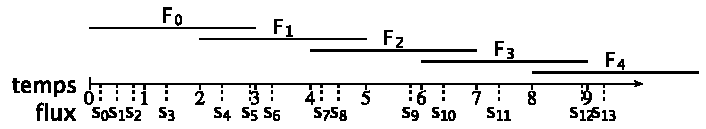
\includegraphics[width=0.7\textwidth]{contrib-astral-fenetres}
	\caption{Séquence de fenêtre de taille $3s$ glissante de $2s$}\label{fig:contrib:astral:fenetres}
\end{figure}

\begin{defi}[Exclusions de bornes de fenêtres]\label{def:exclufenetre}
    Soit $S$ un flux et $(\alpha,\beta,\gamma)$ une description de séquence de fenêtre,

    Les notations $S]\alpha,\beta,\gamma]$, $S[\alpha,\beta,\gamma[$ et $S]\alpha,\beta,\gamma[$ désignent les définitions de l'opérateur classique de séquence de fenêtre permettant d'exclure respectivement les bornes inférieures, supérieures ou les deux.
\end{defi}

\begin{example}
    En reprenant la définition de fenêtre sur 5 secondes : $(j*5s+t_0,j*5s+5s+t_0,5s)$. Nous remarquons que les fenêtres 0 et 1 contiennent les n-uplets dont le \textit{timestamp} est égal à $t_0+5s$. Ainsi, l'opérateur $S]jr+t_0,jr+r+t_0,r]$ avec $r=5s$ permet de retirer les n-uplets à ce \textit{timestamp} de cette fenêtre.
\end{example}

\subsubsection{Fenêtres partitionnées}
L'opérateur de fenêtres partitionnées est très utilisé pour appliquer la même séquence de fenêtres à des sous-flux. Les opérateurs partitionnés sont tous décrits de la même manière. Le principe, illustré dans la figure~\ref{fig:contrib:astral:partition} est de diviser le flux suivant un (ou des) attribut $A$ donné. Sur chacun de ces sous-flux est appliqué un opérateur quelconque. Le résultat est l'union des résultats de ces opérateurs.

\begin{figure}[ht]
	\centering
	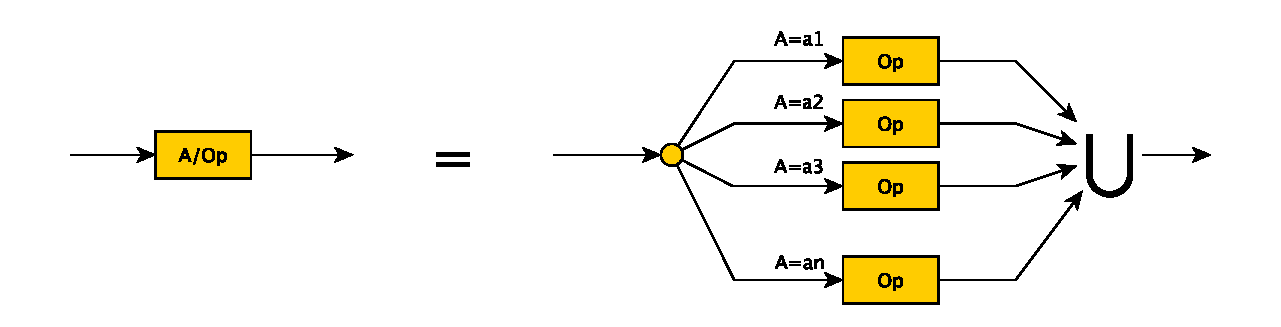
\includegraphics[width=0.9\textwidth]{contrib-astral-partition}
	\caption{Principe d'un opérateur partitionné}\label{fig:contrib:astral:partition}
\end{figure}

Ainsi, nous décrivons dans la définition~\ref{def:partition} de séquence de fenêtre partitionnée l'application de ces principes de partitionnement sur l'opérateur de séquence de fenêtre.
\begin{defi}[Séquence de fenêtre partitionnée]\label{def:partition}
	Soient $S$ un flux, $a_1,...,a_k$ un ensemble d'attributs du schéma de $S$, et $(\alpha,\beta,\gamma)$ une DSF,
	
	Soit $\cup^*$ l'union relationnelle conservant les identifiants physiques, 

	Alors, la séquence de fenêtres $(\alpha,\beta,\gamma)$ partitionnées par $a_1,...,a_k$ est définie par :
	$$S[a_1...a_k/\alpha,\beta,\gamma] = \mathop{\bigcup\null^*}_{a\in Dom(a_1,...,a_k)} (\sigma_{(a_1,...,a_k)=a} S)[\alpha,\beta,\gamma]$$
\end{defi}

Nous remarquons que nous utilisons la définition de l'union relationnelle conservant les identifiants physiques présentés dans la section précédente, ainsi l'ordre naturel décrit dans le flux d'entrée peut être retrouvé dans la relation de sortie.
\begin{example}
	L'exemple le plus courant est la représentation de l'état actuel d'un système à partir d'un flux. Supposons un flux d'entrée $CPU(appId,cpu,\t)$, nous donnant les relevés de charge de processeur. Soit la description de fenêtre rapportant le dernier n-uplet d'un flux : $(1j,1j,1)$. Nous pouvons obtenir la relation temporelle représentant pour chaque application $appId$, la dernière valeur connue de $cpu$ ainsi que le \textit{timestamp $\t$ de mesure} : $$CPU[appId/1j,1j,1]$$

	Cet exemple illustre comment nous pouvons passer d'un flux brut à une représentation (dynamique) d'un \textbf{contexte}. 
	
	La définition du partitionnement par l'union conservant les identifiants physiques permet d'avoir un ordre clair et intuitif sur la relation temporelle résultante. Lorsqu'un nouveau n-uplet entre dans cette relation (ou remplace l'ancien n-uplet), alors il est mis en bout. Avec l'union classique, il est nécessaire de définir l'ordre d'application des unions. Et les n-uplets auraient changé d'identifiants à chaque nouvel état de la fenêtre, ce qui est difficile à contrôler et à manipuler.
\end{example}

Par la suite, plusieurs notations simplifiées sont utilisées pour désigner des descriptions de fenêtres courantes décrites dans le tableau~\ref{tab:windows}.
\begin{table}[ht]
\centering
\begin{tabular}{c||p{0.4\textwidth}|p{0.4\textwidth}}
  & Définition & Équivalence \\ \bottomrule
 $[L]$ & $[j,j,1]$ &  \\ 
 & \multicolumn{2}{p{0.8\textwidth}}{La séquence de fenêtre où chaque fenêtre ne contient que le dernier n-uplet du flux. Cette séquence est égale à $[B]$ si le flux répartit ses n-uplets avec un n-uplet par \textit{batch}.} \\ \hline
 $[B]$ & $]\tau_S^{-1}(\tau_S(j)^-),j,1]$ & $\{s\in S, \BS(s) = \tau_S\circ\tau_S^{-1}(b)\}$ \\ 
 & \multicolumn{2}{p{0.8\textwidth}}{Séquence de fenêtre où chaque fenêtre contient le dernier \textit{batch}.} \\\hline
 $[\infty]$ & $[0,j,1]$ & $\{s\in S, \BS(s) \leq b\}$ \\
 & \multicolumn{2}{p{0.8\textwidth}}{Séquence cumulative contenant tout le flux jusqu'au \textit{batch} courant.} \\\hline
 $[T\ r\ s]$ & $]\max(sj-r+t_0,t_0),sj+t_0,s]$ &  \\
 & \multicolumn{2}{p{0.8\textwidth}}{Fenêtre temporelle de taille $r$ se déplaçant toutes les $s$ unités de temps.} \\\hline
 $[P\ r\ s]$ & $]\max(sj-r,0),sj,r]$ &  \\
 & \multicolumn{2}{p{0.8\textwidth}}{Fenêtre positionnelle de taille $r$ n-uplets se déplaçant tous les $s$ n-uplets.} \\
 \toprule
\end{tabular}
\caption{Liste des fenêtres courantes} \label{tab:windows}
\end{table}
Il est important de noter que les équivalences citées sont non triviales, des démonstrations formelles sont fournies en annexes~\ref{misc:fenetres}.

\subsection{Streamers}
La classe des \textit{streamers} est l'ensemble des opérateurs produisant un flux à partir d'une relation. Son utilisation, après l'application d'une fenêtre, permet la création d'un flux résultant. La définition des streamers est découpée en deux parties, d'abord la définition de la réécriture de \textit{timestamp} qui permet d'ajouter le \textit{timestamp} aux données produites, et ensuite la définition de l'opérateur.
\subsubsection{Réécriture de \textit{timestamp}}
Il est nécessaire de gérer les identifiants physiques. En effet, si un n-uplet est envoyé plusieurs fois dans le flux résultat, il y a conflit si $\varphi$ n'est pas modifié. De plus, tout flux doit avoir un attribut $\t$. Cet attribut doit être créé ou remplacé pour assurer l'hypothèse des ordres. Le principe est que le n-uplet $s\in R(b)$ doit être envoyé dans le flux au \textit{batch} $(t_s,i_s)$, alors nous devons envoyer le n-uplet $\Psi_b(s,t_s)$ décrit dans la définition~\ref{def:stamping}.
\begin{defi}[Fonction de réécriture de \textit{timestamp}]\label{def:stamping}
    Soit $R$ une relation de schéma $A$, $b$ un batch,

    Soit $\I^S = \TN\times \I_R$ le $\Phi$-espace ordonné de manière naturelle,

    La fonction de réécriture de \textit{timestamp} appliquée à $R(b)$ est définie par : 
$$\forall s\in R(b), \ \forall t_s\in\T, \ \Psi_b(s,t_s) = \{(\t,t_s), (\varphi, (b,s(\varphi)))\}\bigcup_{a\in A\backslash\{\varphi,\t\}}\{(a,s(a))\}$$
\end{defi}

Cette définition assure que les nouveaux n-uplets du flux vérifient les propriétés suivantes : 
\begin{itemize}
 \item Ils ont pour \textit{timestamp} $t_s$ le moment où il a été estampillé.
 \item Ils ont un identifiant physique (et du coup une position) plus grand que les identifiants précédents.
 \item L'ordre positionnel de $R(b)$ est préservé.
\end{itemize}
Nous pouvons définir des \textit{streamers} dit sensibles dans la définition~\ref{def:streamers}). Ces \textit{streamers} réagissent aux changements de $R$ et produisent un flux en conséquence.
\begin{defi}[\textit{Streamers} sensibles]\label{def:streamers}
    Soit $R$ une relation,

    Les \textit{streamers} sensibles sont les opérateurs créateurs d'un flux $S$ défini à partir des changements de $R$, trois types sont définis :
\begin{itemize}
 \item Le \textit{streamer} d'insertion, envoyant les nouveaux n-uplets : $\IS(R)$, $$s\in R(t,i) \wedge s\not\in R((t,i)^-) \equ s'=\Psi_{(t,i)}(s,t)\in S \wedge \BS(s') = (t,i)$$
 \item Le \textit{streamer} de suppression, envoyant les n-uplets disparus : $\DS(R)$, $$s\not\in R(t,i) \wedge s\in R((t,i)^-) \equ s'=\Psi_{(t,i)^-}(s,t)\in S \wedge \BS(s') = (t,i)$$
 \item Le \textit{streamer} d'envoi, envoyant tous les n-uplets présents : $\RSu(R)$, $$s\in R(t,i) \neq R((t,i)^-) \equ s'=\Psi_{(t,i)}(s,t)\in S \wedge \BS(s') = (t,i)$$
\end{itemize}
\end{defi}

Nous avons constitué la chaîne complète permettant de traiter les flux de données : flux vers relation, relation vers relation, et relation vers flux. Nous allons explorer un exemple complet pour montrer la clarté d'expression issue de l'algèbre.

\begin{example}
    Le flux d'alerte avec pour attributs (deviceId, avgcpu, $\t$) représente que l'équipement \textbf{deviceId} au \textit{timestamp} $\t$ a eu une charge moyenne \textit{avgcpu} supérieure à 25\%. La moyenne est calculée sur 5 min toutes les minutes.

    Pour former ce flux, il est nécessaire de joindre le flux \textbf{CPU} avec \textbf{Applications} afin de pouvoir associer le bon \textit{deviceId} à l'\textit{appId}. Or, cette opération est interdite à moins de faire une fenêtre sur le flux. Nous pourrions utiliser une fenêtre telle que le dernier \textit{batch} $[B]$, mais comme il est nécessaire d'obtenir une fenêtre temporelle pour le calcul de moyenne, nous pouvons appliquer la description appropriée : $$CPU[T\ 5min\ 1min]\Join Applications.$$

    Appliquons l'opération d'agrégation sur cette relation pour obtenir la moyenne. Puis nous pouvons sélectionner les n-uplets la moyenne est supérieure à 25\%. Enfin, le flux doit être créé à partir de la relation temporelle représentant les équipements supérieurs à 25\% de charge pendant les 5 dernières minutes. Ici une ambiguïté réside dans l'énoncé. Souhaitons-nous avoir le flux des nouveaux équipements ayant ce problème ou souhaitons-nous être notifiés à chaque vérification ? Ce critère va influencer le choix du \textit{streamer} : $\IS$ ou $\RSu$. Prenons le premier, nous obtenons la requête suivante : 
    $$\IS\left(\sigma_{avgcpu \geq 25} \ \null_{deviceId}\G_{avg_{cpu}^{avgcpu}} (CPU[T\ 5min\ 1min]\Join Applications)\right)$$
\end{example}

D'autres streamers peuvent être construits pour effectuer l'insertion de données dans le flux résultat de manière périodique comme le présente la définition~\ref{def:rsr}.
\begin{defi}[\textit{Streamers} périodiques]\label{def:rsr}
    Soit $R$ une relation,

    Les \textit{streamers} périodiques sont les opérateurs créateurs d'un flux $S$ où les insertions ont lieu périodiquement. Le \textit{streamer} $\RS{r}$ est défini par un taux temporel $r$ et la propriété :
$$s\in R(t,i) \wedge t-t_0\equiv 0[r]\equ s'=\Psi_{(t,i)}(s,t)\in S \wedge \BS(s') = (t,i)$$
\end{defi}

Nous avons maintenant défini des opérateurs permettant de couvrir la plupart des opérations. Toutefois, deux opérateurs sont encore à définir pour certaines opérations plus particulière.
\subsection{Manipulation temporelle}\label{sec:contrib:astral:manipulation}
Contrairement à l'algèbre relationnelle, les relations sont temporelles ici. Elles changent au cours de l'exécution de la requête. Il n'existe pas d'opérateurs capables de contrôler ces changements. L'opérateur de manipulation temporelle permet de sélectionner, pour l'instant présent, un état passé d'une relation. Tout d'abord, définissons une transformation temporelle avec la définition~\ref{def:transformation} permettant de sélectionner l'instant voulu sur la relation temporelle. La seule contrainte de cette transformation est l'impossibilité de regarder dans le futur. Nous pouvons ainsi définir l'opérateur de manipulation temporelle (def~\ref{def:manipulation}) qui applique cette transformation à la relation temporelle.
\begin{defi}[Transformation temporelle]\label{def:transformation}
    Une transformation temporelle est une fonction de $\TN\to\TN$ telle que $\forall b\in\TN, f(b) \leq b$.
\end{defi}

\begin{defi}[Opérateur de manipulation temporelle]\label{def:manipulation}
    Soient $R$ une relation, $c$ une condition sur $\TN$ et $f$ une transformation temporelle,

    Alors l'opérateur de manipulation temporelle est défini par $$\D_c^f(R) = b \mapsto \begin{cases} R(f(b)) & \textrm{ si } c(b) \\ \emptyset & \textrm{ sinon}\end{cases}$$
\end{defi}

Plusieurs fonctions classiques ont une utilité directe :
\begin{itemize}
 \item $\mathrm{freeze}^{t_s}(t,i)=(t_s,0)$ si $t \geq t_s$. Permet de figer une relation temporelle à un instant précis, plus aucun changement n'est retransmis à partir de ce point. La relation résultante de cette opération est notée $R^{t_s}$. Un cas particulier est lorsque $t_s=t_0$. Dans ce cas la relation n'a qu'un seul état. Grâce à cette opération, nous sommes capables de faire une \textbf{interrogation instantanée} sur des relations temporelles.
 \item $\mathrm{period}^r(t,i)=\left(\left\lfloor\frac{t-t_0}{r}\right\rfloor r + t_0, 0\right)$ met à jour la relation de manière périodique avec un taux de rafraîchissement $r$.
 \item $\mathrm{change}_S(t,i)=\tau_S\circ\rtau_S$ met à jour la relation à chaque fois qu'un \textit{batch} est inséré dans $S$. Le même principe permet une mise à jour \textit{à chaque fois que la relation $R'$ change}.
\end{itemize}

Cette dernière fonction a un impact particulier lors de la jointure de deux relations temporelles. Dans la jointure (ou au sens large le produit cartésien) telle que nous l'avons définie, si un changement est appliqué d'un côté ou de l'autre, un nouveau calcul de jointure est effectué. Ce comportement peut ne pas être souhaité dans la pratique où nous pourrions souhaiter que seule une branche soit déclencheur de calcul et l'autre soit passive. La jointure semi-sensible permet cette opération. Dans la définition~\ref{def:ssjoin} le résultat $R_1 \ssjoin R_2$ n'est pas mis à jour au changement de $R_2$ mais au changement de $R_1$ avec l'état de $R_2$ correspondant.

\begin{defi}[Jointure semi-sensible]\label{def:ssjoin}
    Soient $R_1$ et $R_2$ deux relations temporelles,

    Soit $\mathrm{change}_{R_1}$ la transformation temporelle telle que $\mathrm{change}_{R_1}(b)$ correspond au dernier changement de $R_1$ inférieur ou égal à $b$,

    La jointure semi-sensible est définie par :
        $$R_1\ssjoin R_2 = R_1 \Join \D^{\mathrm{change}_{R_1}}(R_2)$$
\end{defi}
\begin{example}
    $$DeviceCPU=\IS(\Pi_{deviceId,deviceName,cpu}(CPU[B]\Join Applications)\ssjoin Devices)$$

Le flux résultat $DeviceCPU$ correspond au flux \textit{CPU} originel sur lequel nous avons remplacé l'attribut \textit{appId} par les attributs \textit{deviceId} et \textit{deviceName} qui sont plus intéressants d'un point de vue de l'observation. Si \textit{Devices} est mise à jour (pour changer son statut) en utilisant la jointure simple, la relation temporelle change d'état. Ce qui provoque l'envoi d'un nouveau n-uplet dans le flux. L'opérateur de jointure semi-sensible empêche ce cas puisque les mises à jour sont cadencées par celles de $CPU[B]\Join Applications$ c'est-à-dire $CPU[B]$ soit encore les \textit{batchs} de $CPU$ et non la relation \textit{Devices}.
\end{example}

\subsection{Spread}
Enfin, le dernier opérateur est celui évoqué lors de la conception des \textit{batchs} dans~\cite{Jain:spread}. Il est nécessaire d'avoir un opérateur pour manipuler les \textit{batchs} afin de modifier la fonction $\BS$ d'un flux sans toucher à ses données.

L'opérateur de réinitialisation des \textit{batchs} (def~\ref{def:spreadall}, \textit{spread all} dans la littérature) permet de rassembler les \textit{batchs} multiples pour chaque \textit{timestamp} en un seul. Ceci permet de réorganiser le flux.
\begin{defi}[Réinitialisation des batch]\label{def:spreadall}
Soit $S$ un flux,

Le flux $S$ réinitialisé noté $\lhd S$ vérifie :
$$\forall s\in S, \textrm{ alors } s \in \lhd S, \textrm{ et }\B{\lhd S}(s) = (s(\tau),0)$$
\end{defi}

L'opérateur \textit{spread} décrit dans la définition~\ref{def:spread} permet de découper les \textit{batchs} présents dans un flux en plusieurs nouveaux. Le découpage se fait sur l'ordre induit par ses attributs. Ceci permet par exemple de partitionner selon un identifiant.
\begin{defi}[\textit{Spread}]\label{def:spread}
Soient $S$ un flux de schéma $A$, et $a$ un attribut de $S$,

Soit $\I^S = \TN\times \I_R$ le $\Phi$-espace ordonné de manière lexicographique,

Alors le flux $S$ raffiné par l'attribut $a$ noté $\rhd_{a} S$ vérifie :
$\forall s_1, s_2\in S^2, \textrm{ alors } s_1', s_2' \in (\rhd_a S)^2,$ tel que :
\begin{eqnarray*}
b_1=\B{\rhd_a S}(s_1') < b_2=\B{\rhd_a S}(s_2') &\equ & \BS (s_1) < \BS (s_2)\\ & & \quad \vee \ \left(\BS (s_1) = \BS (s_2)\right. \\ & & \quad\quad \quad\quad\wedge \ \left.s_1(a) < s_2(a)\right)
\end{eqnarray*}

Ainsi que $s_i' = \{(\varphi, (b_i,s_i(\varphi)))\}\bigcup_{x\in A\backslash\{\varphi\}}\{(x,s(x))\}$, pour $i\in\{1,2\}$
\end{defi}

Originellement, si pour l'opérateur \textit{spread}, aucun attribut n'est mentionné, alors tous les n-uplets sont étalés dans des batchs séparés de manière non déterministe. Dans notre algèbre, l'attribut $\varphi$ et l'ordre positionnel permettent de définir l'ordre des \textit{batchs} comme l'ordre positionnel : $\rhd = \rhd_\varphi$. À l'inverse, en appliquant $\lhd$, nous définissons l'ordre des \textit{batchs} comme l'ordre temporel.

\begin{example}
Sachant le contenu du flux \textbf{CPU}(appId, value, $\t$) :

\begin{center}\noindent\begin{tabular}{|c|c|c|} \bottomrule
(1,0) & (1,1) & (2,0) \\ \hline
\begin{tabular}{c}
$(1,20,1)$ \\
$(1,25,1)$ \\
$(2,22,1)$ \\
\end{tabular} &
\begin{tabular}{c}
$(4,10,1)$ \\
$(1,25,1)$ \\
$(4,12,1)$ \\
\end{tabular} &
\begin{tabular}{c}
$(2,23,1)$ \\
$(6,64,1)$ \\
\end{tabular} \\ \toprule
\end{tabular}
\end{center}

 $\lhd\ CPU$ : L'application de l'opérateur de réinitialisation des \textit{batchs} regroupe tous les n-uplets simultanés dans le même \textit{batch}.
 
\begin{center}\noindent\begin{tabular}{|c|c|} \bottomrule
(1,0) & (2,0) \\ \hline
\begin{tabular}{c}
$(1,20,1)$ \\
$(1,25,1)$ \\
$(2,22,1)$ \\
$(4,10,1)$ \\
$(1,25,1)$ \\
$(4,12,1)$ \\
\end{tabular} &
\begin{tabular}{c}
$(2,23,1)$ \\
$(6,64,1)$ \\
\end{tabular} \\ \toprule
\end{tabular}
\end{center}

 $\rhd_{appId}\ CPU$ : L'utilisation du \textit{spread} sur l'identifiant permet d'affiner les \textit{batchs} originels en garantissant que chaque \textit{batch} ne contienne qu'une valeur de \textit{appId}.
 
\begin{center}\noindent\begin{tabular}{|c|c|c|c|c|c|} \bottomrule
(1,0) & (1,1) & (1,2) & (1,3) & (2,0) & (2,1) \\ \hline
\begin{tabular}{c}
$(1,20,1)$ \\
$(1,25,1)$ \\
\end{tabular} &
\begin{tabular}{c}
$(2,22,1)$ \\
\end{tabular} &
\begin{tabular}{c}
$(1,25,1)$ \\
\end{tabular} &
\begin{tabular}{c}
$(4,10,1)$ \\
$(4,12,1)$ \\
\end{tabular} &
\begin{tabular}{c}
$(2,23,1)$ \\
\end{tabular} &
\begin{tabular}{c}
$(6,64,1)$ \\
\end{tabular} \\ \toprule
\end{tabular}
\end{center}

$\lhd\rhd_{appId}\ CPU$ : La combinaison de la réinitialisation et du \textit{spread} permettent d'avoir un \textit{batch} par \textit{timestamp} affecté à une valeur d'\textit{appId}.

\begin{center}\noindent\begin{tabular}{|c|c|c|c|c|} \bottomrule
(1,0) & (1,1) & (1,2) & (2,0) & (2,1) \\ \hline
\begin{tabular}{c}
$(1,20,1)$ \\
$(1,25,1)$ \\
$(1,25,1)$ \\
\end{tabular} &
\begin{tabular}{c}
$(2,22,1)$ \\
\end{tabular} &
\begin{tabular}{c}
$(4,10,1)$ \\
$(4,12,1)$ \\
\end{tabular} &
\begin{tabular}{c}
$(2,23,1)$ \\
\end{tabular} &
\begin{tabular}{c}
$(6,64,1)$ \\
\end{tabular} \\ \toprule
\end{tabular}
\end{center}
\end{example}

Nous avons maintenant présenté l'ensemble des opérateurs de l'algèbre Astral. Nous sommes désormais capables d'exprimer une requête continue (et instantané avec l'aide de la manipulation temporelle) avec une grande clarté et sans ambiguïté sémantique. Nous allons maintenant, définir l'équivalence de requête avec des \textit{timestamps} de départs $t_0$ différents.
\section{Transposabilité}\label{sec:contrib:astral:transposabilite}
Dans la définition de l'équivalence de requête (def~\ref{def:equivalence}), nous avions spécifié le fait que les entités étaient toutes deux initialisées à un \textit{timestamp} $t_0$. Ce type d'équivalence permet de réécrire une requête avant de l'exécuter tout en conservant exactement son comportement. Toutefois, si nous souhaitons nous comparer avec une requête déjà en exécution, la requête ne sera pas synchronisé au même moment. Vu que nous devrons intégrer des données provenant de différentes parties, cet aspect a une grande importance.
\subsection{Équivalence de requêtes multitemporelle}
Afin d'illustrer le fait que l'idée d'effectuer des équivalences de requêtes à différents moments n'est pas trivial, prenons un exemple. Prenons la requête $CPU[B]$. Cette requête représente la relation contenant le dernier \textit{batch} du flux \textbf{CPU}. Dans cette requête, durant la période $[t_0,\tau_S(0)[$, par définition, la relation est vide, c'est à dire : il est nécessaire d'attendre le premier n-uplet avant de former le résultat. Si nous prenons une autre requête ayant démarré au timestamp $t_1 \ll t_0$. Alors pendant la période $[t_0,\tau_S(0)[$, lui sera plein. Ceci constitue un exemple de ce que nous appelerons le phénomène d'élaboration (def~\ref{def:elaboration}.
\begin{defi}[Phénomène d'élaboration]\label{def:elaboration}
    Le phénomène d'élaboration correspond à une période initiale de la vie d'une requête durant laquelle le résultat n'est pas calculable. Cette période transitoire constitue l'élaboration d'une requête.
\end{defi}

Ainsi, nous sommes capable d'établir l'équivalence entre deux requêtes (def~\ref{def:equivalencegenerale}) si effectivement les résultats sont équivalents à partir d'un certain moment. Pour cela, nous définissons qu'il existe un \textit{timestamp} pour lequel, l'initialisation des entités (grâce à $\sigma$ et $\D$) à celui-ci impliquera une équivalence des résultats.
\begin{defi}[Équivalence de requêtes générale]\label{def:equivalencegenerale}
    Soient $(Q_1(E_1),t_1)$ et $(Q_2(E_2),t_2)$ deux requêtes quelconques,

    Soit $\E_t$ l'opérateur égal à $\begin{cases} \sigma_{t\geq \t} & \textrm{ si les requêtes sont des flux}\\ \D_{t\geq \t}^{(t,i)} & \textrm{  si les requêtes sont des relations}\end{cases}$

    Alors l'inclusion de requêtes entre ces requêtes est définie par $$\exists t \in \T, \textrm{ tel que } \quad (\E_t\ Q_1(E_1), t_1) \subseteqq (\E_t\  Q_2(E_2), t_2)$$

    L'équivalence de requêtes est définie par double inclusion.
\end{defi}

Nous avons donc défini une notion générique d'équivalence. Voyons désormais les conséquences du changement de \textit{timestamp} d'initialisation pour une requête donnée.
\subsection{Transposabilité}
La transposabilité (def~\ref{def:transposabilitereq}) est le fait de changer le \textit{timestamp} de départ d'une requête.
\begin{defi}[Transposabilité de requête]\label{def:transposabilitereq}
    Soit $(A,t_0)$ une requête,

    $A$ est transposable par $B$ sur $T\subseteq \T$ si et seulement si : $$\forall t\in T, \quad (A,t_0) \equiv (B,t)$$

    $A$ est dite \textit{naturellement} transposable si $B=A$.
\end{defi}
Toutefois, cette définition ne fait pas avancer la résolution du problème car nous ne sommes pas capable a priori de calculer la transposition de la requête sur son nouveau \textit{timestamp}. Pour permettre la résolution de ce problème, nous allons raisonner par récursivité sur les opérateurs. Chaque opérateur peut se transposer (def~\ref{def:transposabiliteop} en un autre sur un ensemble de \textit{timestamp} calculé.
\begin{defi}[Transposabilité d'opérateur]\label{def:transposabiliteop}
    Soit $O$ un opérateur unaire,

    Soit $(Q,t_0)$ une requête transposable par $Q'$ sur $E$,

    $O$ est un opérateur transposable par $O'$ sur $T$ si et seulement si : $$(OQ,t_0) \textrm{ est naturellement transposable par } O'Q' \textrm{ sur } T\cap E$$

    $O$ est dit \textit{naturellement} transposable si $O'=O$.
\end{defi}

Afin d'avancer dans notre réfléxion. Il est absolument nécessaire d'initialiser notre récurrence en supposant (car rien ne le présage) que pour toute expression algébrique : il est possible de trouver un ensemble d'entité source naturellement transposable. D'un point de vue de l'exécution, cela veut dire que nous ne contrôlons pas directement les sources de données. Ainsi, les entités sources ne sont pas influencé sur le moment où le démarre une requête qui les exploite.
\begin{hyp}[Transposabilité native]\label{hyp:transposabilite}
    Soit $(Q(E),t_0)$ une requête,

    Alors il existe une expression $Q'(E')$ telle que : $$\forall A\in E', \qquad A \textrm{ est naturellement transposable sur } \T$$
    
    Les éléments de $E'$ sont appelés sources de la requête.
\end{hyp}
Cette affirmation reste toutefois à travailler car lors du déploiement d'une requête, nous instantions aussi le processus d'acquisition, qui est lui dépendant du moment de démarrage. Nous explorerons ces aspects lors de l'exploration de l'expressivité d'Astral dans le chapitre~\ref{chap:validation:expressivite}.

\begin{example}\label{ex:transposabilite}
	En tant qu'exemple, afin d'illustrer les propriétés de transposabilité, nous allons explorer la transposabilité d'une requête simple. Supposons que nous souhaitons obtenir la transposabilité de la requête permettant d'obtenir toutes les 5 secondes la liste des dispositifs actuellement connectés dans la maison : $\RS{5s} (\sigma_{deviceStatus=1} Devices)$. 
	
	Ici, nous supposons par l'hypothèse des transposabilités des sources que $Devices$ est naturellement transposable à tout instant. La sélection par la suite est un opérateur qui a la particularité de ne traiter que l'instant présent et est donc naturellement détaché de toute dépendance à $t_0$. Donc $\sigma_{deviceStatus=1} Devices$ est naturellement transposable à tout instant aussi.
	
	Par contre, $\RS{r}$, lui n'est pas transposable à tout moment. En effet, dans sa définition la condition d'appartenance au flux produit est la suivante : $s \in R(t,i)\wedge t-t_0 \equiv 0[r]$. Ainsi, si nous transposons à $t_1$, pour obtenir équivalence des requêtes, il faut que $\forall t \geq t_1$, $t-t_0\equiv t-t_1\equiv 0[r]$.  Ce qui nous conduit à montrer que $t_1 = t_0 +kr$ avec $k\in \Z$. 
	
	Supposons que $t_1$ vérifie cette condition. Nous arrivons très facilement à voir que $\forall R$, en prenant $t=\max(t_1,t_0)$, nous avons bien\footnote{en suivant naturellement les définitions, nous obtenons de plus une égalité stricte même sur les $\varphi$} que $(\E_{t}\RS{r}(R),t_0) \equiv (\E_{t}\RS{r}(R),t_1)$. Donc :
	\begin{center}$\RS{5s}\sigma_{deviceStatus=1} Devices$ est naturellement transposable sur $\{t\in \T /\ t\equiv t_0 [5s]\}$\end{center}
\end{example}

Nous avons désormais exploré comment nous pouvions faire des équivalences de requêtes à travers le temps et comment manipuler ces concepts pour en extraire des propriétés. Dans la chapitre~\ref{chap:validation:expressivite}, nous explorons des cas généraux et plus complexe de transposabilité pour démontrer la puissance d'expression d'Astral.

\section{Conclusion}
Ce chapitre a dressé un état de l'art des différents systèmes capables d'offrir une solution générique de supervision. Il en ressort qu'aucun système ne supporte entièrement les critères de qualité que nous nous sommes fixés. Le tableau~\ref{tab:rw:supervision:bilan} résume les 11 points d'analyse en colorant les différentes points suivant leurs conformités. 

\begin{sidewaystable}[ht]
\centering
\begin{tabular}{@{{\vrule width 1pt}\ \ }>{\raggedleft}m{3cm}@{\ \ {\vrule width 1pt}\ \ }M{4.2cm}|M{4.2cm}|M{4.2cm}|M{4.2cm}@{\ \ {\vrule width 1pt}}} \bottomrule
\head Critère & \head Système d'administration & \head Gestion de contexte & \head Entrepôts de données & \head Gestion de flux de données \\  \toprule \bottomrule
\critereAA & Hiérarchique & Triplets & Relationnel & Relationnel dérivé \\ \hline
\critereAB & \meh Structure hiérarchique sans contraintes & \good Ontologies & \good Modèle relationnel normalisé & \bad Pas de structure \\ \hline
\critereAC & \meh Notifications & \bad Ajout du temps en propriété & \meh CDC & \good Flux natif \\ \toprule \bottomrule
\critereBA & \meh Instantanée, continu en ad-hoc & \bad Instantané principalement & \meh Instantané. ETL en pseudo-continu & \bad Continu uniquement \\ \hline
\critereBB & \good Standardisation, union de modèles & \meh Fusion d'ontologies non standardes & \good Processus ETL (complexe) & \good Union et jointures de flux \\ \hline
\critereBC & \bad Impératif principalement & \good Logique & \meh Déclaratif (SQL) et Procédural (ETL) & \good Déclaratif principalement\\ \hline
\critereBD & \meh Procédures à écrire soi-même & \good Logique du premier ordre & \good Relationnel multidimensionnel et Algorithmie dédiée & \meh Relationnel avec support du dynamisme\\ \toprule \bottomrule
\critereCA & \good Support des standards & \meh Spécification longue des domaines & \bad Spécification du schéma, des ETL, autre (complexe) & \good Écriture de requêtes \\ \hline
\critereCB & \bad Aucune & \good Séparation par les domaines & \good Données multidimensionnelles & \bad Aucune \\ \hline
\critereCC & \good Modèle extensible, fonctions métiers dans le gestionnaire & \meh Capteurs virtuels & \good Opérateurs ETL, procédures SQL, algorithmes & \meh Sources et puits mais pas les opérateurs  \\ \hline
\critereCD & \good Large échelle & \bad Complexité très haute & \meh Réactivité lente, Support de grande quantité & \good Support de haut débits\\ \toprule 
\end{tabular}
\caption{Récapitulatif de l'état de l'art des systèmes génériques de supervision}\label{tab:rw:supervision:bilan}
\end{sidewaystable}
Il en ressort que les systèmes d'administrations sont avant tout des systèmes qui fonctionnent grâce au support des standards et à leur simplicité d'implémentation. L'architecture avec gestionnaire adaptable grâce à des langages impératifs permets une grande flexibilité pour s'adapter aux cas d'usages. De son côté, l'informatique contextuelle fournit des outils permettant de modéliser et manipuler proprement les concepts du système grâce aux ontologies et aux raisonnements logiques. Il en sort une claire séparation des domaines de compétences. Les entrepôts de données quant à eux se distinguent par des capacités d'analyses très poussées, ainsi qu'un procédé d'intégration, très complexe et lourd malheureusement, mais très complet. Enfin, la gestion de flux de données est une base solide pour gérer les données dynamiques. L'intégration et l'adaptation au système étant fait entièrement de manière déclarative en fait une solution performante et viable.

À la vue de l'état de l'art, voici les points qui vont être critique sur notre établissement de notre contribution :
\begin{itemize}
    \item La gestion de flux est un bon socle pour gérer les données dynamique grâce aux requêtes continues.
    \item Elle ne suffit pas pour constituer un système d'observation complet, notamment à l'absence de modèle de description et de requêtes instantanées.
    \item Les entrepôts et bases de données sont capables de répondre aux requêtes instantanées.
    \item Les ETL sont trop complexes à manipuler pour intégrer les données, alors que les SGFD sont plus déclaratifs.
\end{itemize}
Il devient clair que les systèmes de gestions de flux de données forment un bon candidat comme fondation pour un architecture d'observation de système. Il nous faut donc approfondir l'état de l'art technique sur ce domaine pour modeler notre contribution. Le point majeur sera d'apporter les capacités des systèmes de gestions de données relationnels. En effet, en apportant le support persistant à la gestion de flux de données, en clarifiant et augmentant son langage, nous aurons un outil qui sera plus apte à répondre à notre problématique. Ainsi, l'héritage du relationnel permettra une structure sémantique correcte, ainsi que des capacités d'analyses plus évoluées. Enfin et surtout, les données serait intégrés malgré leur hétérogénéité profonde. Le chapitre suivant détaille l'état de l'art technique de la gestion de flux de données afin de pouvoir effectuer ces améliorations.
